\begin{figure}[tbp]
\centering
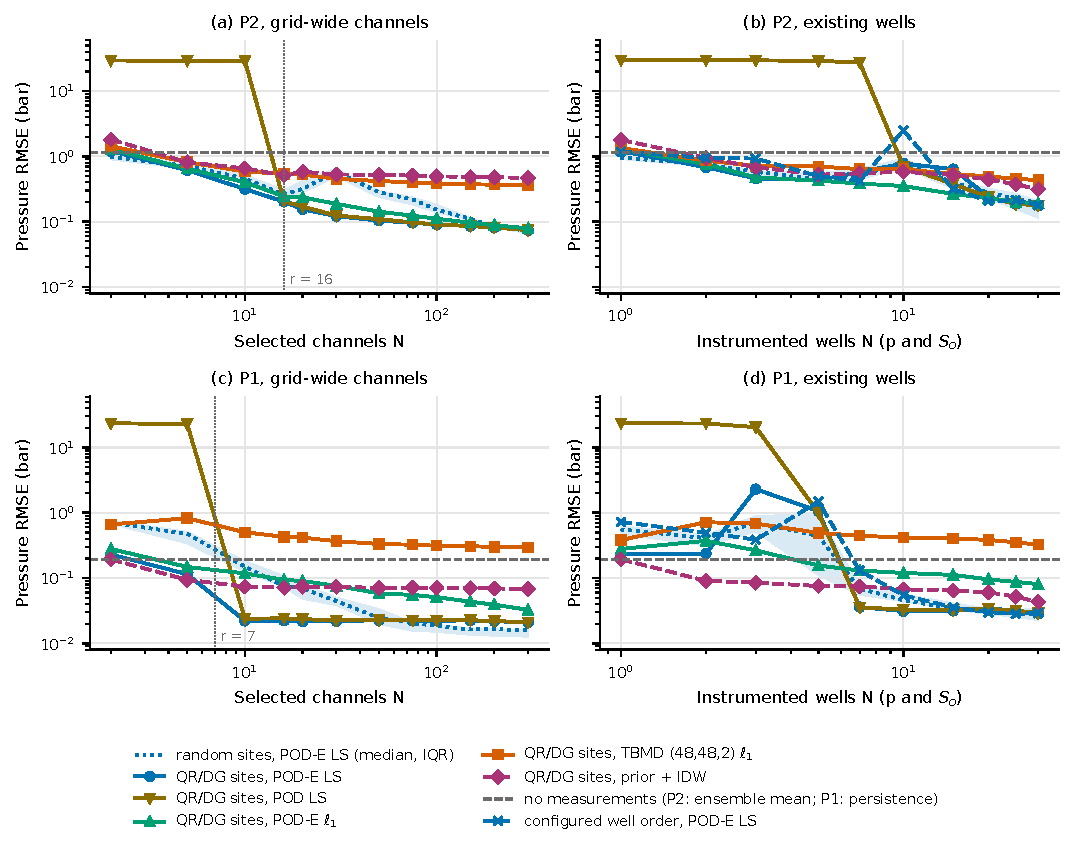
\includegraphics[width=\textwidth]{../../../../studies/brugge_sparse_sensing/figures/fig4_budget_curves.pdf}
\caption{Pressure RMSE (supplied export unit $u_p$; mean over ten folds) against the measurement budget. (a) P2, grid-wide channels; (b) P2, existing wells measuring pressure and $S_o$; (c, d) the same for P1. QR: pivoted-QR/determinant-greedy channels; DG: determinant-greedy well order; both computed on the basis named in the legend. The shaded band and dotted line show the interquartile range and median over folds of the per-fold median of 20 random placements (POD-E, LS). Dashed grey: no-measurement reference; vertical dotted line: dictionary depth $r$. Axes are logarithmic; standard deviations are given in Table~\ref{tab:main}.}
\label{fig:budget}
\end{figure}
